\shipout\null
\newpage
\chapter*{Summary}
\addcontentsline{toc}{chapter}{Summary}
Outside our earth various kinds of events take place which we wish to 
observe: Black hole outbursts, supernovae, cosmic jets, ...
These events produce various kinds of messengers which are useful to obtain
information on the event: Gravitational waves, gamma rays, protons,...
But one particle within this set of particles is quite unique and
the subject of our study: The neutrino. 

The neutrino is unique in that it points back to the event itself.
Due to the neutrino not having any charge, nearly no mass and 
interacting weakly it doesn't get bent nor absorbed and re-emitted 
on it's way to us unlike, say, the proton. This means that if we observe
a neutrino back here on earth it's very likely that the direction we observe
it in is the direction it came from.

We wish to detect a particular type of neutrinos: The ultra high energy (UHE)
neutrino.  There have been lots of neutrino detectors around but none of them
have been able to observe \textit{cosmogenic neutrinos} which would live past
the 3 PeV energy range. This is probably caused by the exponentially falling
flux with increasing energy, implying that a really big detector volume is
required to detect neutrinos with such high energies. 

Due to cost requirements, it was necessary to work in the radio regime.  As
much as we'd like a really big detector working in the visible spectrum, it
would cost way too much. As neutrinos can produce radio waves upon interacting
in ice through the Askaryan effect and as radio waves can travel for way longer
distances in there before interacting than visible light, it was previously
decided in experiments like ARA and ARIANNA to detect on the principle of
radio waves. The Radio Neutrino Observatory in Greenland or RNO-G which is
currently under construction and the subject of this thesis builds on the
knowledge of these experiments to make a quite complex detector which
should be capable of detecting UHE neutrinos.

The ice properties have an impact on how radio waves propagate. As mentioned before, RNO-G is a detector built
in the Greenland icecap. As the radio waves get produced in the ice we need to figure out how
they propagate towards our detector. An important part in figuring out how they propagate is 
the local index of refraction which seems to be linearly related to the density of the ice. 
The density of the ice seems to vary continuously with depth. A function describing
this overall relation of the index of refraction with the depth is called an \textit{ice model}
and it is crucial for future studies to understand this ice model.

As previously said index of refraction in ice has been assumed to follow a linear relationship with 
the density through Schytts equation:
\begin{equation*}
  n(z) \approx 1 + 0.78\frac{\rho(z)}{\rho_0}
\end{equation*}
The indices of refraction vs depth that got computed this way are shown in figure \ref{fig:SumFinRes}
in gray, throughout the RNO-G project the ice model that got used was the one single exponential shown in 
green.

Due to the ice model seeming to deviate from the theoretically expected single
exponential, it was necessary to develop a new algorithm to find the paths the
radio waves could take with more complex ice models.  The software used within
this thesis to figure out the path radio waves take is called
\textit{radiopropa}.  Even though this software can be used to work with most
kinds of ice models, it still needs to be used within some kind of algorithm to
be useful. Such an algorithm has already been developed called the
\textit{Iterative ray tracer} as is explained in section \ref{sec:Iterative}
but it had its shortcomings, that's why in this thesis a new algorithm was
developed called the \textit{hybrid ray tracer} which is explained in chapter
\ref{chapter:hybrid}. The hybrid ray tracer makes it possible to both find a
more accurate solution and find it faster. The accuracy of the ray tracer
is showcased in figure \ref{fig:SumHyb}, the Iterative ray tracer can
be considered it's predecessor and it's accuracy is shown in figure \ref{fig:Sumit}
showcasing the clear improvement.

\begin{figure*}
	\centering
\begin{minipage}{0.49\textwidth}
	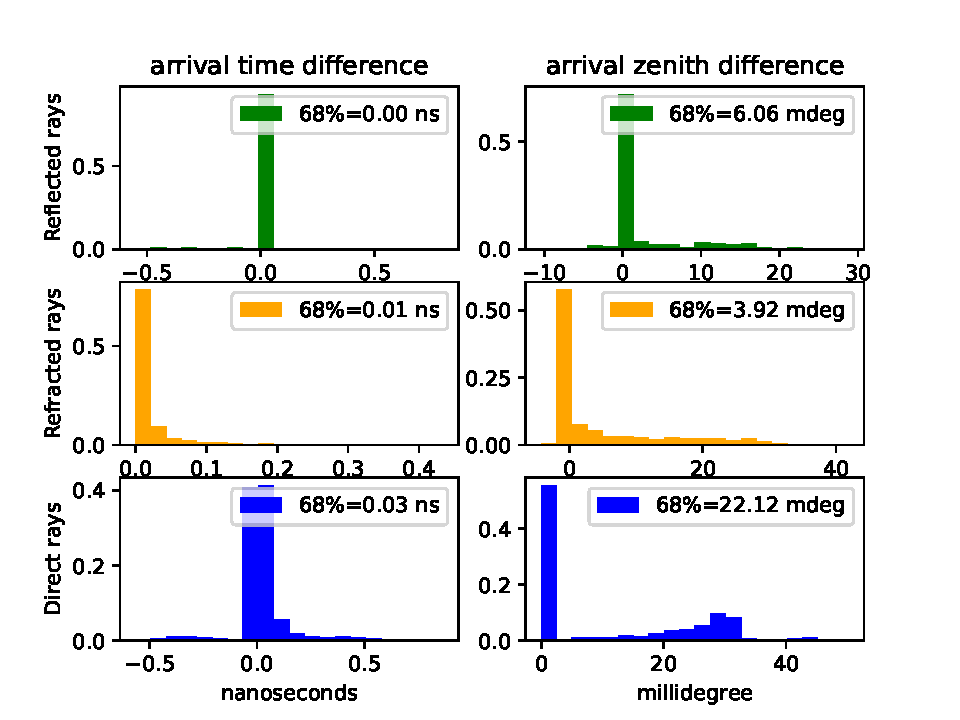
\includegraphics[width=1.1\textwidth]{figures/hybrid_comparison_N_1000.pdf}
	\caption{Hybrid}
	\label{fig:SumHyb}
\end{minipage}
\begin{minipage}{0.49\textwidth}
	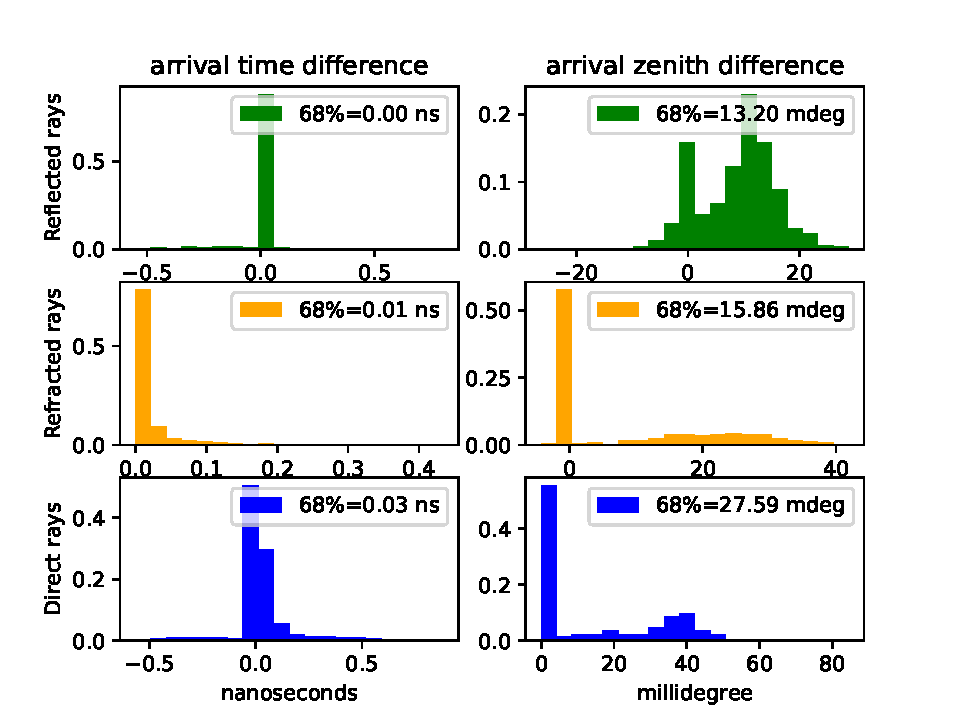
\includegraphics[width=1.1\textwidth]{figures/iterative_comparison_N_1000.pdf}
	\caption{Iterative}
	\label{fig:Sumit}
\end{minipage}
\end{figure*}

\newpage
It is, however, crucial to make sure we actually need a new kind of ice model.
The measuring of the index of refraction can be accomplished indirectly through
weather balloon fly-byes as is explained in chapter \ref{chap:WB}. Every day in
the summer, two times per day a weather balloon is launched from the base camp.
This weather balloon is equipped with an antenna which sends out a 403MHz
sinusoidal signal, upon close fly-byes with detectors this signal can be
observed in the detectors (as is visualized on the cover). By looking at the
difference in arrival time of the signal, the difference in timing can be made
out from which a plane wave reconstruction can be done. As this plane wave
reconstruction is heavily dependent on the local index of refraction in the
ice, it can be indirectly measured through this reconstruction.  After this
analysis the following data was found:
\begin{center}
\begin{tabular}{||c c c c c c||}
 \hline
 Depth (m) & Station id & channels & Run:Event & n$_\text{exponential}$ & n$_\text{fit}$\\ [0.5ex]
 \hline\hline
 -94.518 & 11 & 0\&2\&3 & 1034:12397 & 1.7397 & 1.7045 $\pm$ 0.006 \\
 \hline
\end{tabular}
\end{center}
\begin{figure}
	\centering
	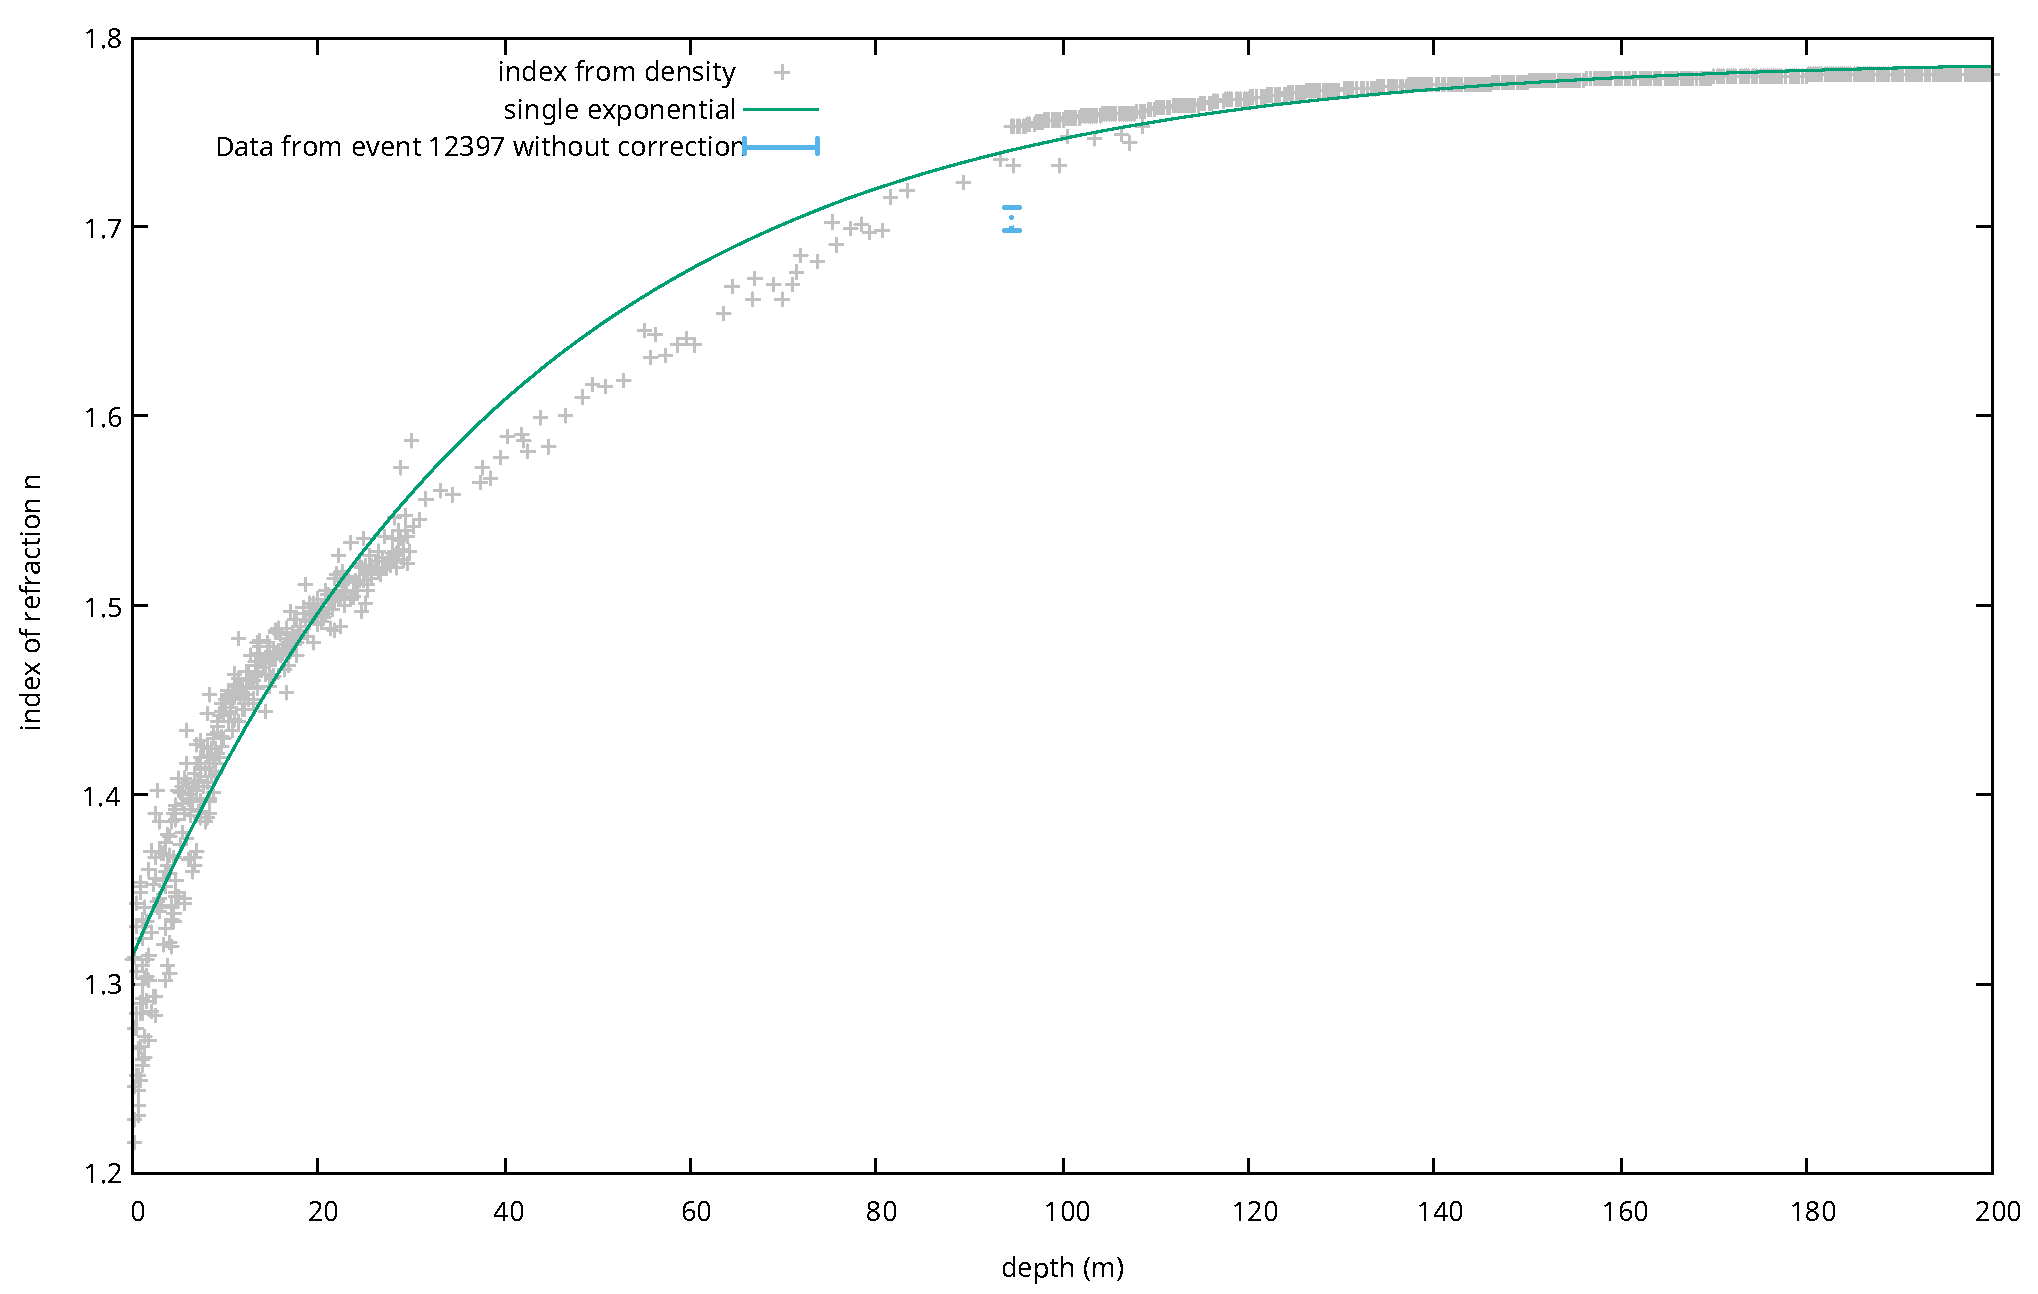
\includegraphics[width=0.9\textwidth]{figures/Event12397NoCorr.pdf}
  \caption{Event 12397 shows itself as a clear outlier hinting at the need to investigate the index-depth relation further}
  \label{fig:SumFinRes}
\end{figure}
And visually shown as the data in blue on figure \ref{fig:SumFinRes}, 
it clearly shows a big discrepancy with the exponential model.
We reason that this clearly shows that there's a need to investigate
the index-depth relation further as the wave propagation, and thus
neutrino reconstruction, are heavily dependent on the ice model.
\newpage
\chapter*{Samenvatting}
\addcontentsline{toc}{chapter}{Samenvatting}
Er vinden verscheidene gebeurtenissen plaats in het heelal waarover we
meer wensen te weten zoals Black hole outbursts, supernovae, cosmic jets,...
Al deze gebeurtenissen produceren vormen van informatie dewelke we kunnen
infereren door hun op een manier te detecteren zoals de protonen en fotonen
maar ook meer exotische bronnen van informatie zoals zwaartekracht golven.
Maar één bepaald deeltje vinden wij bijzonder interessant: de neutrino.

De neutrino heeft als erg unieke eigenschap dat het terugwijst naar het event
waar ze gecreëerd werd. In tegenstelling tot andere deeltjes zoals protonen
heeft de neutrino geen lading, bijna geen massa en interageert ze zeer zwakjes.
Door deze eigenschappen zal ze op de weg naar de aarde niet afgebogen worden 
door magneetvelden en hoogstwaarschijnlijk niet interageren met tussen media zoals
gaswolken. Deze eigenschappen impliceren dat, als we erin slagen een neutrino te detecteren, de 
richting waarin ze gedetecteerd wordt hoogstwaarschijnlijk eenzelfde richting is als
waar ze vandaan komt.

Neutrino's komen in verscheidene energieën voor maar wij zijn geïnteresseerd in één bepaald gebied,
boven de 3 PeV oftewel de ultra hoge energie (UHE) neutrino. In de verscheidene experimenten die 
neutrino's hebben gedetecteerd is er nog geen een in geslaagd neutrino's te observeren met 
energieën boven de 3 PeV. Dit is het regime waar zich zogenaamde \textit{cosmogenic neutrinos} zouden
bevinden en dus uiterst interessant om te bestuderen. Maar, om zo'n hoge neutrino energie waar te nemen,
blijkt een zeer grote detector nodig te zijn.

Aangezien het zeer snel zeer duur zou zijn om een voldoende grote detector te bouwen om deze neutrino's 
te detecteren in het visuele spectrum, wat bijvoorbeeld gebruikt wordt in detectoren zoals IceCUBE,
werd besloten om te leunen op het Askaryan effect. Dit is het effect dat zorgt voor de productie
van radiogolven bij interactie van een neutrino in ijs. Aangezien radio golven verder vrij kunnen
propageren in ijs dan zichtbaar licht maakt dit het mogelijk om de verscheidene antennes verder
van elkaar te plaatsen. Enkele experimenten zijn op dit principe gebouwd zoals ARA en ARIANNA.
Uit de expertise van deze en soortgelijke experimenten werd dan de Radio Neutrino Observatory in Greenland of RNO-G gemaakt.
RNO-G moet het mogelijk maken om UHE neutrino's te observeren en deze thesis wenst bij te dragen tot de ontwikkeling
van deze detector.

Het blijkt dat de eigenschappen van het ijs een effect hebben op hoe radiogolven zich propageren door het ijs.
Aangezien RNO-G gebouwd is in Groenland op een groot volume ijs en ze werkt op het principe van radiogolven
is het nodig dit te onderzoeken. Het blijkt dat de propagatie sterk afhankelijk is van de locale refractieve
index van het ijs, dewelke lineair lijkt gerelateerd te zijn aan de dichtheid van het ijs. Hoe de locale
refractieve index afhangt van de ruimtelijke positie wordt het \textit{ijs model} genoemd. Theoretisch
verwacht men een exponentiële afhankelijkheid van de dichtheid met de diepte, maar uit metingen blijkt deze
af te wijken van het theoretische model. 

De ray tracing simulaties die gebruikt worden om na te gaan waar de neutrino
vandaan komt zijn sterk afhankelijk van het ijs model.  Er werd vroeger een
algoritme gemaakt dewelke enkel met het exponentieel model kan omgaan, maar
door de recent gevonden tekortkomingen aan dit ijs model bleek het nodig een
nieuw algoritme te bedenken. Zo'n algoritme, genaamd de \textit{iterative ray
tracer} werd daarom uitgevonden (zie sectie \ref{sec:Iterative}) maar bleek
enkele tekortkomingen te hebben. Daarom vonden wij het nodig om een nieuw soort
algoritme uit te vinden dewelke steunt op dat algoritme genaamd de
\textit{hybrid ray tracer}, de werking van dit algoritme kan gevonden worden in
hoofdstuk \ref{chapter:hybrid}. Dit algoritme maakt het mogelijk om beide een
meer accurate oplossing te vinden en deze eveneens sneller te vinden.
De accuraatheid van de ray tracer wordt geillustreerd in figuur \ref{fig:SamHyb}
. Hiernaast, in figuur \ref{fig:Samit}, wordt zijn voorganger de iterative ray tracer
getoond. Er is een duidelijke verbetering te zien bij vergelijking van de twee.
\begin{figure*}
	\centering
\begin{minipage}{0.49\textwidth}
	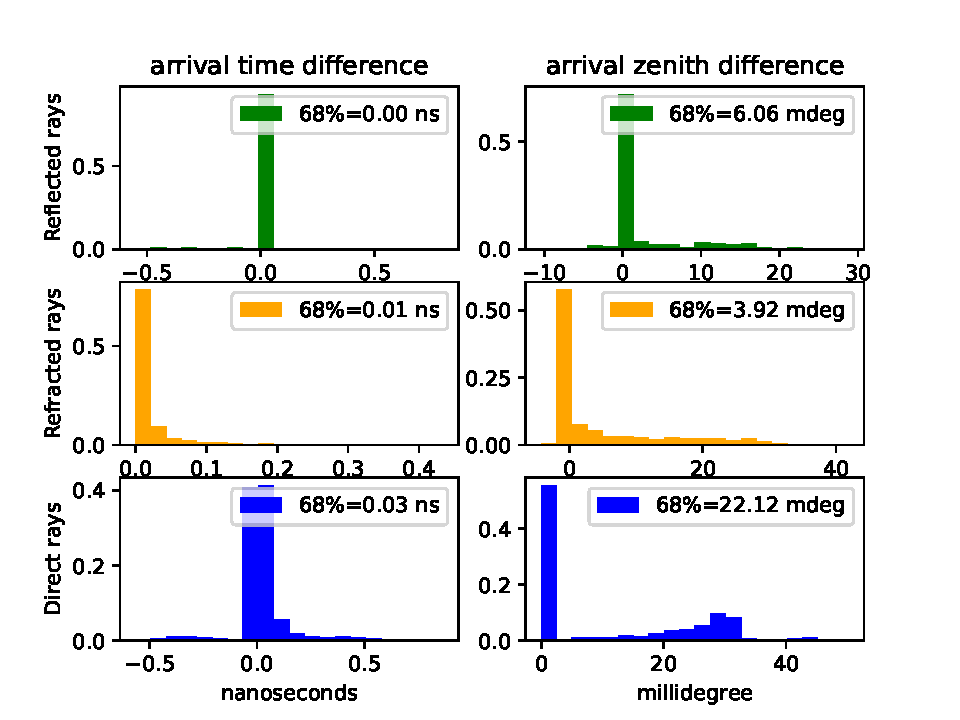
\includegraphics[width=1.1\textwidth]{figures/hybrid_comparison_N_1000.pdf}
	\caption{Hybrid}
	\label{fig:SamHyb}
\end{minipage}
\begin{minipage}{0.49\textwidth}
	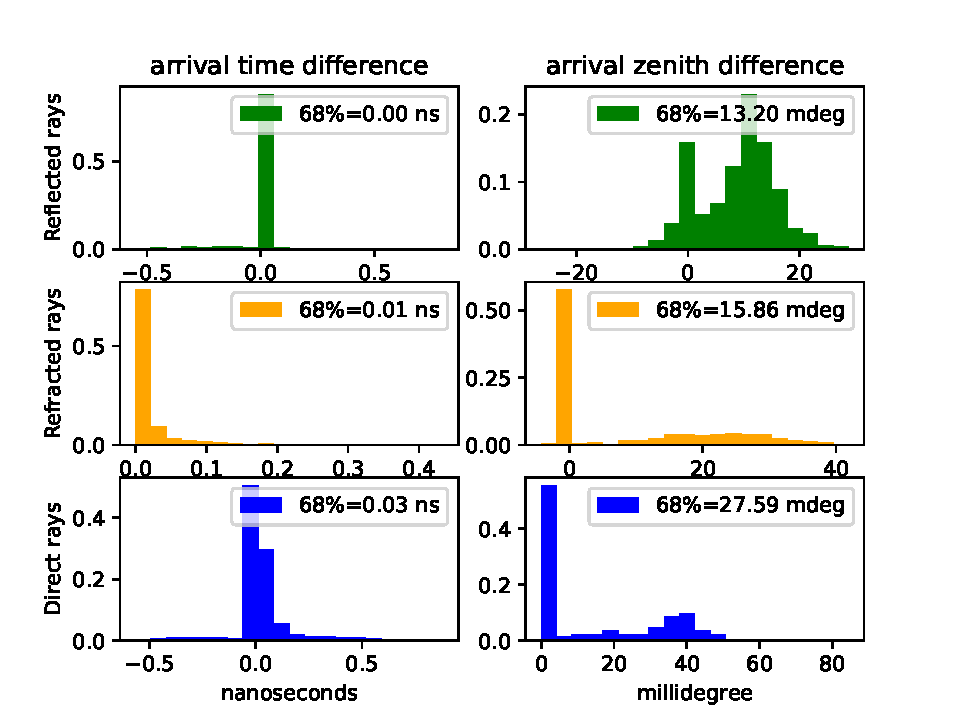
\includegraphics[width=1.1\textwidth]{figures/iterative_comparison_N_1000.pdf}
	\caption{Iterative}
	\label{fig:Samit}
\end{minipage}
\end{figure*}
\newpage
Maar om over te schakelen op een nieuw ijs model met een ander algoritme is het nodig aan te tonen dat er effectief
een groot verschil is tussen het theoretische exponentiële model en de echte refractieindex. Om dit aan te tonen 
kunnen we gebruik maken van weerballonnen. Elke dag in de zomer, 2 maal per dag, wordt een weerballon gelanceerd 
op de RNO-G basis. 
Deze weerballon beschikt over een antenne dewelke een sinusoïde signaal uitstuurt aan 403MHz, als zo'n ballon toevallig
dicht bij een detector komt zal dit signaal kunnen gedetecteerd worden. Door een plane wave reconstructie te doen
van dit signaal en gebruik te maken van de positie van de ballon kunnen we infereren wat de locale refractieve index
is in het ijs. Deze procedure wordt volledig uitgelegd in hoofdstuk \ref{chap:WB}.
Na deze procedure toe te passen werd de volgende data gevonden:
\begin{center}
\begin{tabular}{||c c c c c c||}
 \hline
 Depth (m) & Station id & channels & Run:Event & n$_\text{exponential}$ & n$_\text{fit}$\\ [0.5ex]
 \hline\hline
 -94.518 & 11 & 0\&2\&3 & 1034:12397 & 1.7397 & 1.7045 $\pm$ 0.006 \\
 \hline
\end{tabular}
\end{center}
\begin{figure}
	\centering
	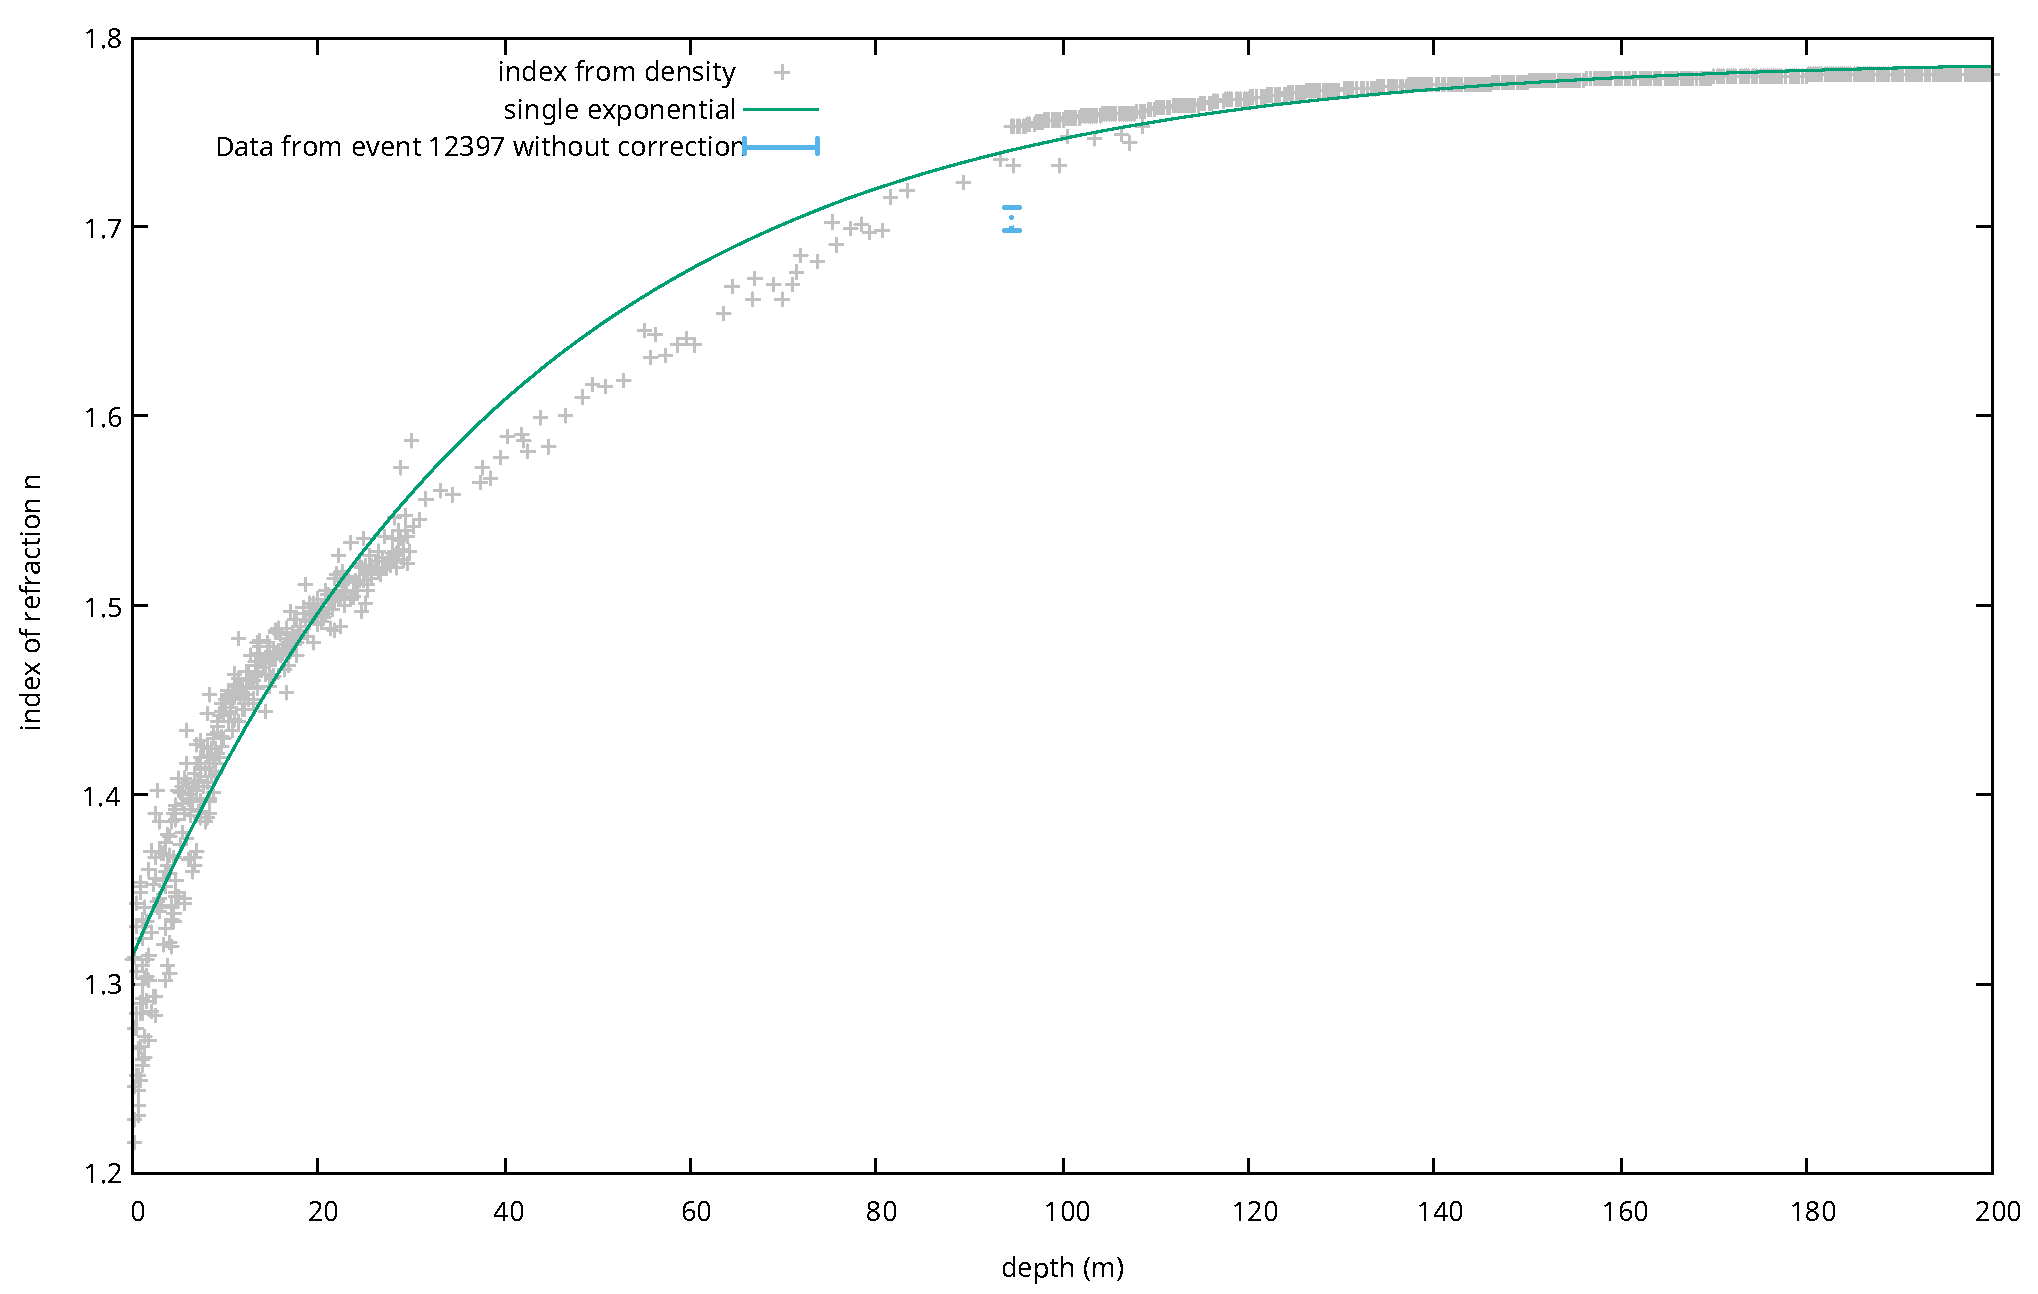
\includegraphics[width=0.9\textwidth]{figures/Event12397NoCorr.pdf}
  \caption{Event 12397 shows itself as a clear outlier hinting at the need to investigate the index-depth relation further}
  \label{fig:SamFinRes}
\end{figure}
Dewelke ook visueel wordt weergegeven in figuur \ref{fig:SamFinRes}, er is een
duidelijk verschil tussen de gemeten index van refractie ($n_{fitted}$) en die
uit het exponentieel model ($n_{exponential}$) te zien.
Wij concluderen dat dit duidelijk toont dat er een nood is om de refractieve index-diepte
relatie verder te onderzoeken aangezien deze de concusies uit neutrino metingen sterk
zal beïnvloeden.
\newpage
\chapter*{Dankwoord}
\addcontentsline{toc}{chapter}{Dankwoord}
Ik zou Prof.Dr.em. Dirk Ryckbosch wensen te bedanken om daar te zijn doorheen
heel mijn studie carrière. Eerst wanneer hij de voorstelling van de richting
Fysica en Sterrenkunde deed in Ledeganck toen ik nog in de humaniora zat. Later wanneer ik buisde op
mechanica maar hij me zei dat, aangezien mijn oefeningen goed waren, ik er
duidelijk wel talent voor had en gewoon meer moest studeren met als afsluiter
"tot in de master". En finaal hier wanneer ik een thesis doe met hem als
promotor.

Ik zou Bob Oeyen willen bedanken om mij altijd te helpen wanneer ik
vragen had. Ook heeft hij mij veel geholpen door kritisch te zijn op
mijn werk en mij zo vooruit te helpen in beide mijn presentaties en
mijn schrijfwerk.

Ik wens mijn ouders te bedanken om altijd daar te zijn voor mij.
Ik apprecieer het nog altijd enorm om te kunnen jetskiën of
tennissen met mijn vader (en binnenkort ook met mijn moeder).
Ook zijn vele inzichten in deze thesis gekomen na even wandelen
met mijn moeder en mijn hond Mickey.  Zonder hen zou ik hier
waarschijnlijk nooit geraakt zijn.

Als laatste wens ik mijn partner Polina te bedanken, zij heeft me
meer dan wie dan ook gesteund en verdient heel mijn hart.
\newpage
% ------------ TABLE OF CONTENTS ---------
{\hypersetup{hidelinks}\tableofcontents} % hide link color in toc
\newpage


